\documentclass[9pt]{IEEEtran}

\usepackage[english]{babel}
\usepackage{graphicx}
\usepackage{epstopdf}
\usepackage{fancyhdr}
\usepackage{amsmath}
\usepackage{amsthm}
\usepackage{amssymb}
\usepackage{url}
\usepackage{array}
\usepackage{textcomp}
\usepackage{listings}
\usepackage{hyperref}
\usepackage{xcolor}
\usepackage{colortbl}
\usepackage{float}
\usepackage{gensymb}
\usepackage{longtable}
\usepackage{supertabular}
\usepackage{multicol}

\usepackage[utf8x]{inputenc}

\usepackage[T1]{fontenc}
\usepackage{lmodern}
\input{glyphtounicode}
\pdfgentounicode=1

\graphicspath{{./figures/}}
\DeclareGraphicsExtensions{.pdf,.png,.jpg,.eps}

% correct bad hyphenation here
\hyphenation{op-tical net-works semi-conduc-tor trig-gs}

% ============================================================================================

\title{\vspace{0ex}
Classification trees, random forests}

\author{Marko Medved\vspace{-4.0ex}}

% ============================================================================================

\begin{document}

\maketitle

\section{Part 1: Implementing multinomial logistic regression and ordinal logistic regression }
\subsection{Implementation details}
The first model implemented is multinomial logistic regression. 
In this approach, we calculate linear predictors for each class, 
excluding the reference class. Afterward, we apply the softmax function
 to compute the probability for the true class. To optimize the model’s 
 weights, we use the maximum likelihood estimation (MLE) method, leveraging 
 the \textit{fmin\_l\_bfgs\_b} optimizer with numerical gradients.
 
An important aspect of this implementation is the inclusion of an 
intercept column. This is necessary because, in some cases, all feature 
values may be zero. Without the intercept, this would lead to zero
 probabilities for all classes. By including the intercept, we ensure 
 that the model can still generate non-zero probabilities for all classes,
  even when the features are zero.

During the prediction phase, we apply the softmax function to the
 linear predictors for each class at each data point. This gives us 
 the predicted probabilities for all classes, which are then reported as
  the model's predictions.  \\

  Next, ordinal logistic regression was implemented. The main difference
   with multinomial logistic regression is the assumption that the target 
   categories have a natural ordering. This assumption allows us to 
   significantly reduce the number of parameters. Instead of calculating
    separate predictors for each class, we use just one linear predictor 
    along with thresholds (which are fewer than the number of classes) to
     determine the boundaries between classes.

  During the model building phase, we again use the MLE approach, as we did with multinomial 
  logistic regression, and the same optimizer. Instead of 
  explicitly modeling the thresholds, we model the differences between
   the thresholds. To ensure numerical stability, we constrain
    these differences (the deltas) to be greater than 1 during the
     optimization process.
  
  This reduction in parameters, combined with the ordered nature 
  of the categories, makes ordinal logistic regression more efficient
   for datasets with ordered categorical targets.

\subsection{Testing our implementation on the basketball dataset}
We evaluated both classifiers on the provided dataset to predict
 shot type based on various features. To preprocess the data, we One-Hot encoded 
 the categorical variables and dropped one category from each feature
  to avoid multicollinearity. Furthermore, we identified strong correlations
   between certain features. Specifically, the "TwoLegged" and "No Movement"
    features, as well as the player type indicators "Guard" and "Forward,"
     exhibited high correlation, which we can observe on Figure~\ref{fig:corr}. As a result, we removed the "TwoLegged" 
     and "Forward" features to prevent convergence problems and reduce 
     redundancy.

The model evaluation was conducted using 10-fold cross-validation, 
and the uncertainty in the results was calculated under the assumption 
of asymptotic normality. The results are presented in 
Table~\ref{tab:results}. As expected the multinomial version outperformed the 
ordinal one, since there is no clear natural order for shot types in 
basketball.


\begin{figure}[h]
    \centering
    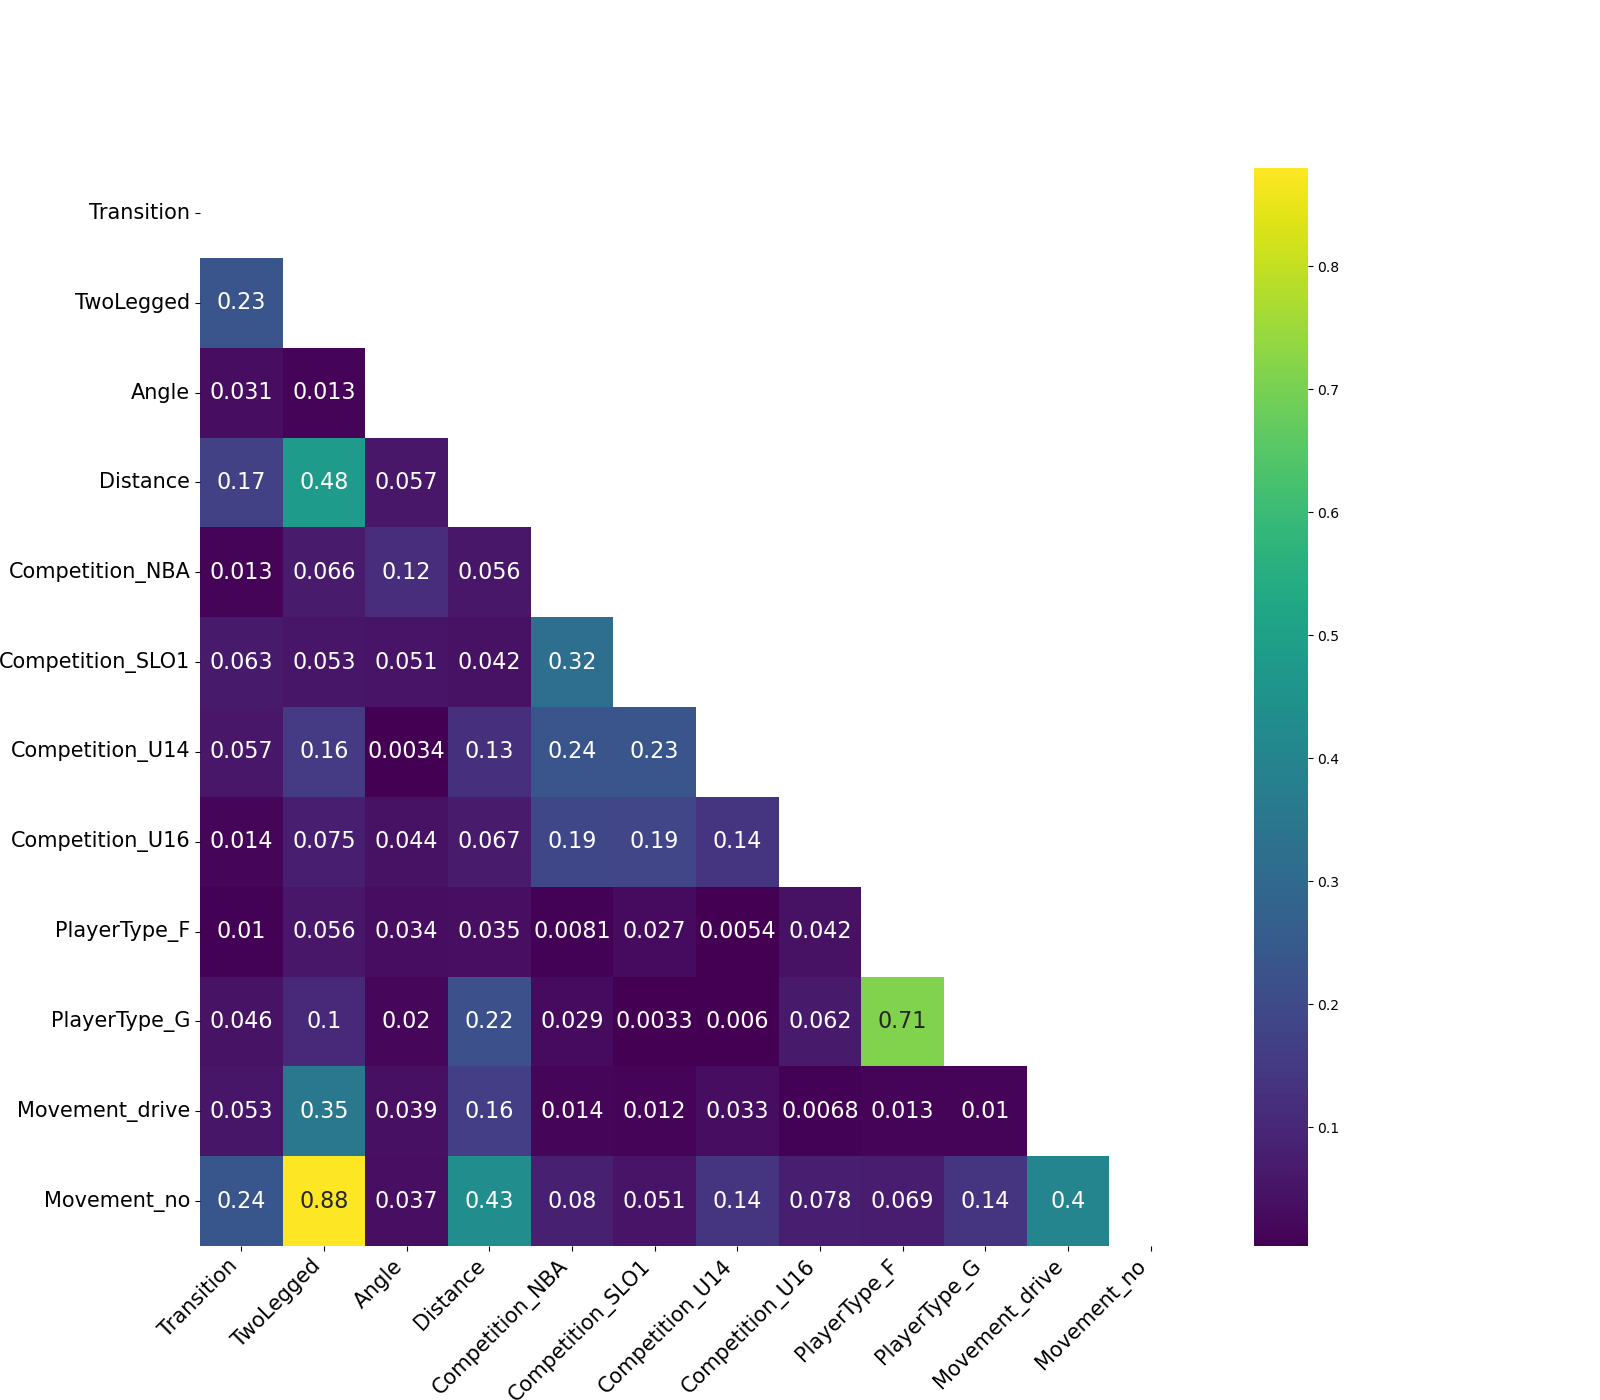
\includegraphics[width=0.99\columnwidth]{figures/corr.png}
    \caption{Absolute correlation of features in the basketball dataset.}
    \label{fig:corr}
\end{figure}

 \begin{table}[h]
    \centering
    \begin{tabular}{l|l|l}
    Model       & Accuracy & Log loss          \\ 
    \hline
    Multinomial  & 0.7353 $\pm$ 0.0062 & 0.667 $\pm$ 0.012 \\
    Ordinal  & 0.7138 $\pm$ 0.0064& 0.985 $\pm$ 0.018\\

    \end{tabular}
    \vspace{2px}
    \caption{Comparison of results using multinomial and ordinal logistic regression}
    \label{tab:results}
\end{table}

\section{part 2.1: Application of the Multinomial regression}
In this analysis, we explored the relationships between shot type and various features.
 To gain insight, we directly compared the coefficients from the linear predictors. These 
 coefficients represent how the log-odds of a given shot type change when a particular feature
  is adjusted, while holding other features constant.\\
To estimate the uncertainty of these coefficients, we employed bootstrap sampling.
 We repeatedly fitted the model to bootstrap samples, calculated the mean of the betas
  as our best estimate, and used the standard deviation as the measure of uncertainty. 
  We used the "tip-in" shot type as our reference class.\\
The results of our analysis are displayed in Figure~\ref{fig:betas}. From the plot, we 
observe that some features exhibit high uncertainty compared to the value of coefficients 
in certain shot types, suggesting that these features may not contribute significantly to 
differentiating those shot types from the reference class. On the other hand, several features
 show consistently high coefficients across multiple shot types.\\
For instance, the "Movement\_no" coefficient is notably influential. The likelihood of no
 movement would intuitevely be high for the "above head" shot. However, this comparison is
  made against the "tip-in" shot, where the only movement in the dataset  is "Movement\_no"—which
   is also true for "dunk" and "hook shot" categories. In contrast, "Movement\_drive" has a clear,
    intuitive impact. For example, a drive is less likely to be associated with an "above head"
     shot but is much more common for "layup" and "other" shots. For the "tip-in", "hook shot", 
     and "dunk", the likelihood of a drive is relatively similar to the reference class.\\
The "Distance" feature also shows an interesting pattern: the "tip-in"(reference) shot is associated with 
the shortest distances, followed by the "dunk", "layup", and "hook shot". Both "other" and 
"above head" shots, on the other hand, have higher coefficients, which aligns with their nature 
(mostly for the above head), as they often occur from farther distances.\\
When examining the "Competition\_U14" feature, we see that "tip-in" is less likely compared
 to all shot types except for the "dunk". This makes sense, as younger players (under 14) are 
 unlikely to perform tip-ins and even less likely to dunk.\\
Finally, the intercept plays a significant role across all shot types. It represents the 
baseline log-odds of selecting a particular shot type when all other features are zero. 


\begin{figure}[h]
    \centering
    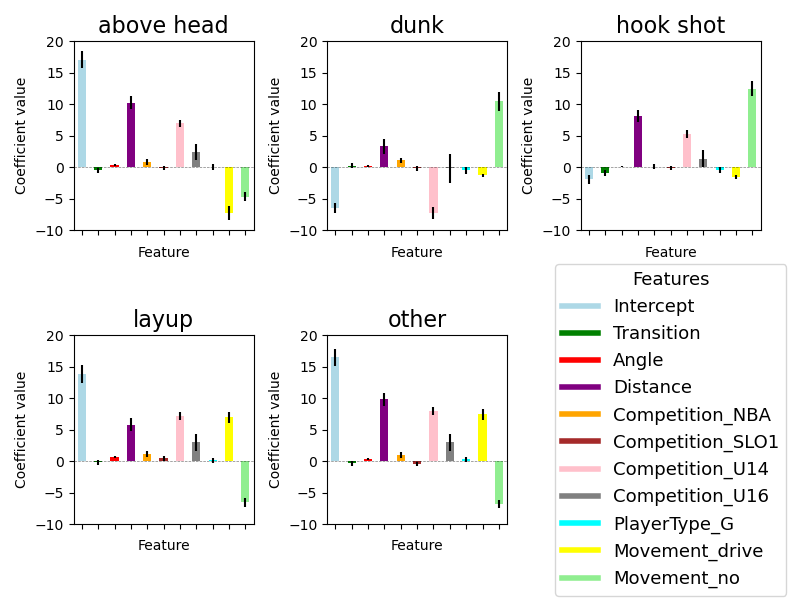
\includegraphics[width=.99\columnwidth]{figures/betas.png}
    \caption{Comparison of relationships of features and different shot types}
    \label{fig:betas}
\end{figure}

\section{part 2.2: Application of the Ordinal regression}
In this section, we designed a data-generating process (DGP) where ordinal
 logistic regression outperforms multinomial logistic regression. The process
  was designed as follows: We begin by assigning a class to each data point.
   For each class, we generate the corresponding feature values by sampling 
   from a uniform distribution spanning from i - 0.5 to i + 0.5, where i is 
   the current class. This ensures that the data is ordinal in nature. To 
   introduce some variability and reduce the correlation between features,
    we then add noise sampled from a standard normal distribution.

We tested the DGP using a dataset with 100 training data points and 100
 testing data points. The results of this experiment can be seen in 
 Table~\ref{tab:logistic_comparison}.


\begin{table}[ht]
    \centering
    \begin{tabular}{l|c|c}
    \textbf{Model} & \textbf{Accuracy} & \textbf{Log Loss} \\
    \hline
    Multinomial Logistic Regression & $0.580 \pm 0.050$ & $0.942 \pm 0.100$ \\
    Ordinal Logistic Regression     & $0.630 \pm 0.049$ & $0.823 \pm 0.070$ \\
 
    \end{tabular}
    \caption{Comparison of accuracy and log loss  between multinomial and ordinal logistic regression models.}
    \label{tab:logistic_comparison}
    \end{table}
    

\section{Part 3: GLM Diagnostics}
In this section, we implemented linear regression under the assumption that the residuals 
follow a normal distribution, utilizing the least squares method. We applied this model to 
predict basketball shot distance based on the shot angle. The results of the fitted linear 
regression can be seen in Figure~\ref{fig:lg}.

Upon examining the residuals, we observe that their distribution is bi-modal, rather than 
normal as we initially assumed. This is not entirely surprising, given that the distribution
 of shot distances, as shown in Figure~\ref{fig:distr}, is also bi-modal. Additionally, the 
 correlation between shot angle and shot distance is very low (-0.056), which further contributes
  to the similar distribution of residuals across all data points. 

  \begin{figure}[h]
    \centering
    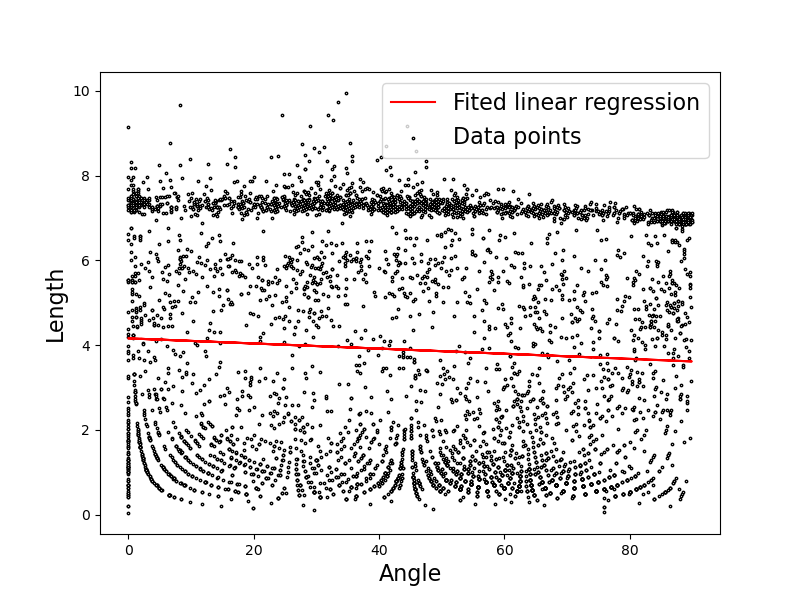
\includegraphics[width=0.99\columnwidth]{figures/lin_reg.png}
    \caption{Linear regression, predicting shot length from shot angle}
    \label{fig:lg}
\end{figure}



\begin{figure}[h]
    \centering
    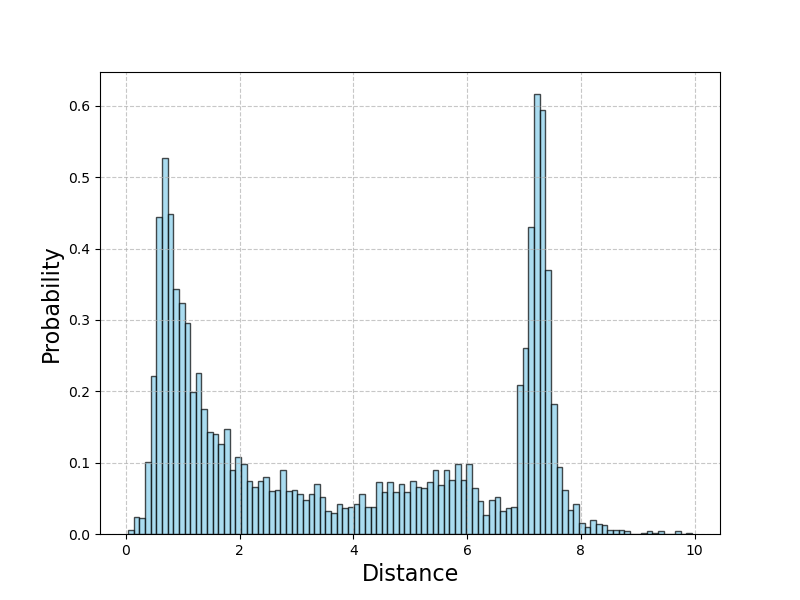
\includegraphics[width=0.99\columnwidth]{figures/distr.png}
    \caption{Distribution of the distance of basketball shots}
    \label{fig:distr}
\end{figure}


As part of our diagnostic checks, we plotted the Q-Q plot
 (Figure~\ref{fig:qq}) to assess whether the assumption of normally
  distributed residuals holds. In the Q-Q plot, we compare the quantile
   residuals (we choose the quantile residuals because they are approximately normally distributed as 
   long as we choose the correct distribution from the exponential family)
    to the theoretical quantiles of a standard normal distribution.
    If the residuals were normally distributed, the points would align closely
     with the reference line. However, as shown in the plot, the residuals
      deviate significantly from this line, indicating that the normality 
      assumption is not justified. Again, from this plot we can see that the disribution 
      of residuals is bi-modal.


\begin{figure}[h]
    \centering
    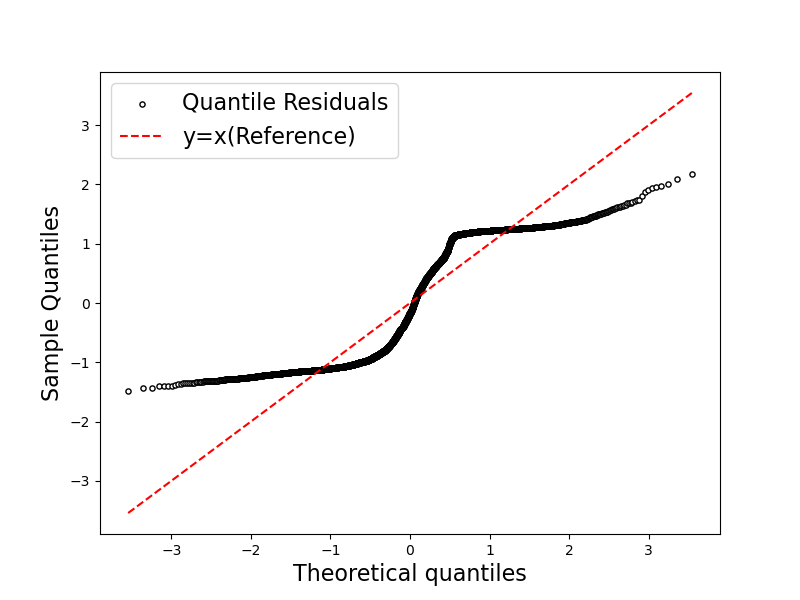
\includegraphics[width=0.99\columnwidth]{figures/qq.png}
    \caption{Quantile-quantile plot}
    \label{fig:qq}
\end{figure}


The second plot is the quantile residuals vs fitted values plot. We chose to use quantile
 residuals because they tend to have approximately constant variance (if we choose the correct 
 distribution), which makes them suitable
  for assessing homoscedasticity. This plot
   helps us verify whether the variance of the residuals changes across the range of fitted values.

In Figure~\ref{fig:res_vs_fitted}, we observe that there is a trend in the residuals by the 
fitted polynomial regression, which shows that linear regression is not a great choice for 
this model. We can also see that the scatter doesn't have a particular pattern that would suggest 
drastically changing variance, so we can assume homoscedasticity. 


\begin{figure}[h]
    \centering
    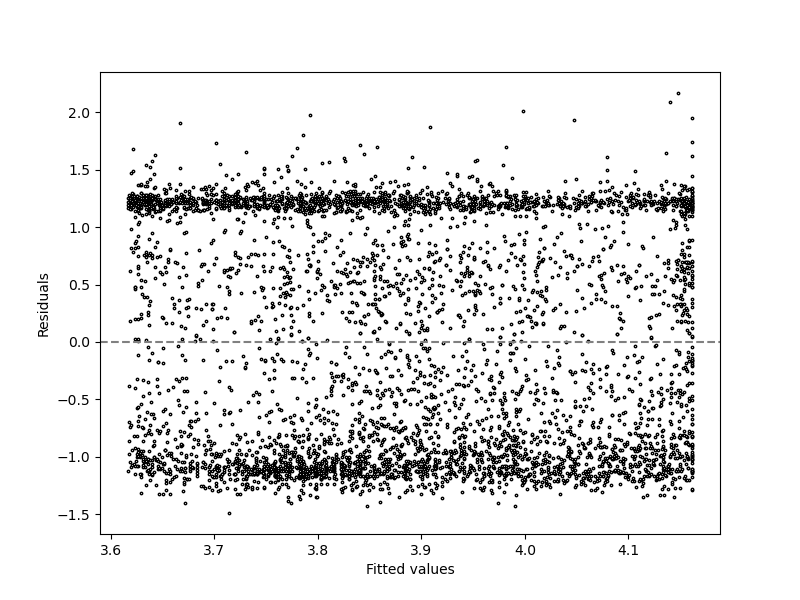
\includegraphics[width=0.9\columnwidth]{figures/res_vs_fitted.png}
    \caption{Residuals vs fitted values}
    \label{fig:res_vs_fitted}
\end{figure}

The last plot, shown in Figure~\ref{fig:cook}, represents Cook's distance for each data point.
 Cook's distance measures the influence of individual data points on the regression model,
  taking into account both the features and the target values. A high Cook's distance indicates
   that a data point has a significant impact on the model, potentially altering the estimated 
   regression coefficients.

In the plot, we observe that none of the points have a particularly high Cook's distance.
 As a rule of thumb, data points with a Cook's distance close to  than 1 are 
 considered highly influential. Since all the points lie way below this threshold, we can 
 conclude that there are no particularly influential data points that would unduly affect 
 the model. Therefore, it is safe to assume that the regression results are not being 
 significantly impacted by any single data point.

\begin{figure}[H]
    \centering
    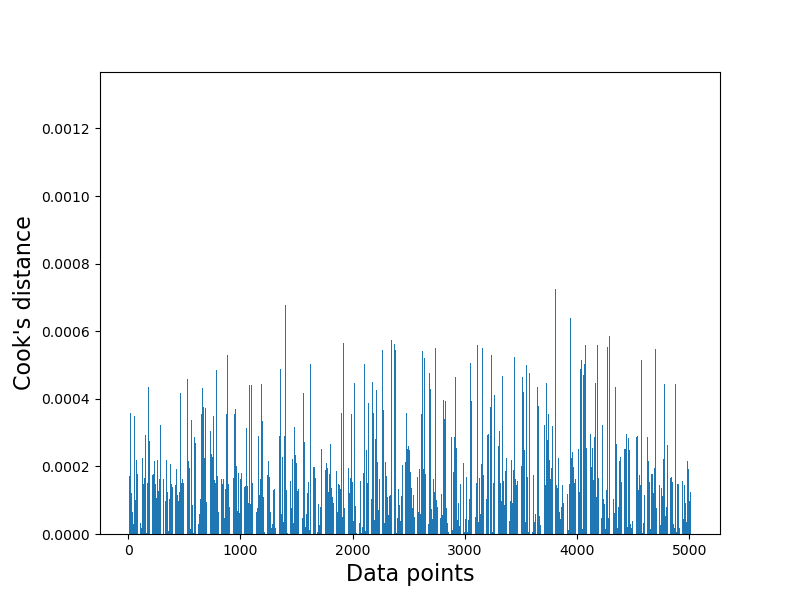
\includegraphics[width=0.9\columnwidth]{figures/cook.png}
    \caption{Cook's distance across data points}
    \label{fig:cook}
\end{figure}

\end{document}
